%!TEX root = ../EmbSW2.tex
\section{CRC}
\subsection{Blockcodes}
\begin{itemize}
	\item	Blockcodes erzeugen aus k Eingangssymbolen (z.B. k Nutzdatenbits) n Ausgangssymbole (z.B. n = k Nutzdatenbits + r redundante Codebits). Ein solcher Code wird (n,k)-Code genannt.
	\item Jeder Block aus k Symbolen wird unabhängig von anderen Blöcken codiert und erzielt für diesen Block ganz spezifische Erkennungs- und Korrekturfähigkeiten.
	\item Ein Blockcode ist linear, wenn die Modulo-2 Addition zweier beliebiger gültiger Codeworte wieder ein neues gültiges Codewort ergibt.
	\item Alle $2^k$ möglichen Blocks der Länge k werden eindeutig auf $2^k$ Codeworte der Länge n abgebildet. Die Auswahl der $2^k$ Codeworte aus der Menge von $2^n$ zur Verfügung stehenden Codeworten ist massgebend für die Fähigkeit, Fehler zu detektieren oder gar zu korrigieren.
\end{itemize}

\subsection{Zyklische Codes}
\begin{itemize}
	\item Zyklische Codes sind eine Untergruppe der linearen Blockcodes. Sie zeichnen sich durch eine einfache Realisierung in Hardware aus, welche bei nicht-zyklischen Blockcodes vor allem bei grossen Blocklängen k und n recht umfangreich wird.
	\item Zyklische Blockcodes sind einerseits als fehlerkorrigierende Codes sehr beliebt, z.B. Hamming-Codes, der Golay-Code, BCH-Codes oder die nicht-binären Reed-Solomon Codes.
	\item Als fehlererkennende Codes sind CRC-Codes in praktisch jedem ausgereifteren Datenübertragungssystem anzutreffen.
\end{itemize}

\subsection{CRC-Codes in Embedded Systems}
\begin{itemize}
	\item Daten auf nicht-flüchtigen Speichern wie Harddisks, Flashspeicher
	\item Übertragung von Programmcode, der in ein Embedded System geladen werden soll
	\item Datenübertragung allgemein, z.B. bei Ethernet (häufig wird bei der Datenübertragung nur Parität verwendet)
	\item Einschränkung: CRC-Codes sind gut für die Kanalcodierung, welche sporadische Fehler wie Rauschen detektieren soll, jedoch sind sie ungeeignet, um systematische Datenmanipulationen festzustellen. Zur Sicherstellung der Datenintegrität müssten kryptographische Verfahren eingesetzt werden.
\end{itemize}

\subsection{Polynomschreibweise}
Bei zyklischen Codes werden zur mathematischen Behandlung Code-Sequenzen addiert, subtrahiert, multipliziert und dividiert (jeweils \textbf{Modulo-2}).\\

\begin{tabular}{|l|c|}
\hline Codewort  & $c = (c_0, c_1, c_2, c_3,$ \dots $, c_{r-1})$ \\
\hline Polynom &  $c(x) = c_0 + c_1 \cdot x + c_2 \cdot x^2 + $\dots$ + c_{r-1} \cdot x^{r-1}$\\
\hline
\end{tabular} \\ \\

\begin{itemize}
	\item Polynom ist von max. Grad (r-1) mit Koeffizienten $c_i$\\
		z.B. $c = (1, 0, 0, 1, 1, 0) \Rightarrow c(x) = 1 + x^3 + x^4$
	\item Die Addition und Subtraktion modulo 2, d.h. ohne Carry, entspricht je einer XOR-Verknüpfung
	\item $M(x) = Q(x) \cdot G(x) + R(x)$
	\begin{itemize}
		\item $G(x)$ : Generator-Polynom
		\item $R(x)$ : Rest-Polynom \qquad $Grad[R(x)] < Grad[G(x)]$
		\item $Q(x)$ : Quotient-Polynom
		\item $M(x)$ : Nachricht-Polynom
	\end{itemize}
	\item Das Generator-Polynom $G(x)$ muss zwischen Sender und Empfänger abgemacht werden
	\item Der Sender berechnet den Rest R(x), der Quotient Q(x) interessiert nicht
	\item Der Sender sendet die Meldung $M(x)$, und hängt den Rest $R(x)$ an, d.h. der gesamte gesendete Block entspricht\\
		$x^{r-1} \cdot M(x) + R(x)$ \qquad	r: Anzahl Bits in $G(x)$
	\item Der Empfänger teilt die Meldung inkl. der Prüfsequenz durch $G(x)$, d.h.
		$[x^{r-1} \cdot M(x) + R(x)] \div G(x)$
	\item Die Meldung ist fehlerfrei angekommen, falls die empfangene Prüfsequenz gleich Null ist
\end{itemize}

\subsubsection{Berechnung der Prüfsequenz R(x)}
\begin{itemize}
	\item $x^{r-1} \cdot M(x)$ bilden, d.h. der Meldung $M(x)$ müssen $(r-1)$ Nullen angehängt werden $=: T(x)$
	\item Diese Bitfolge $T(x)$ durch das Generator-Polynom $G(x)$ teilen
	\item Die angehängten Nullen in T(x) durch R(x) ersetzen und senden.
	\item Auf der Empfangsseite genau die Folge T(x) durch G(x) teilen, der Rest muss Null werden
\end{itemize}

\begin{tabular}{c|c}
	\textbf{Senderseite (CRC Generieren)} & \textbf{Empfängerseite (CRC Decodieren)} \\
	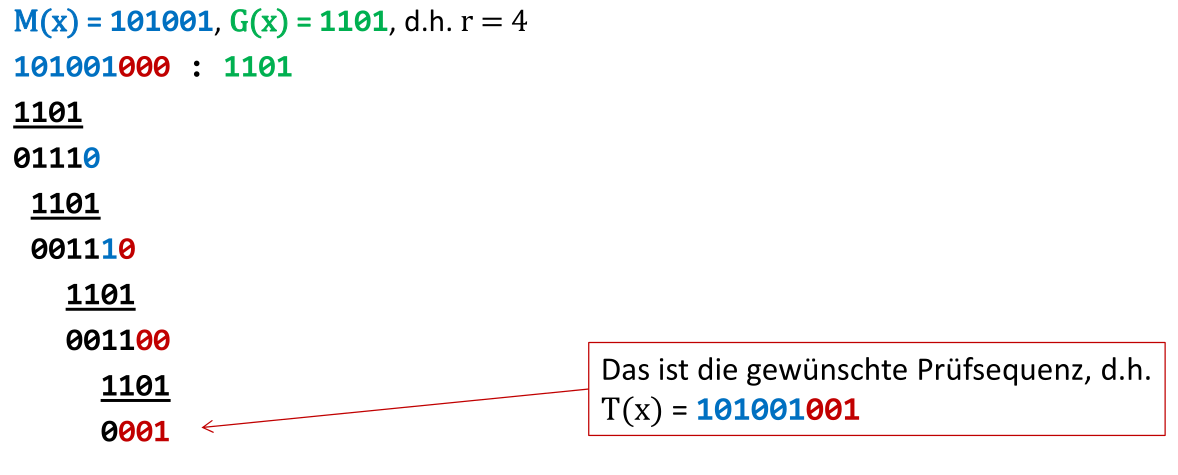
\includegraphics[width=10cm]{images/CRC/crc-gen.png} & 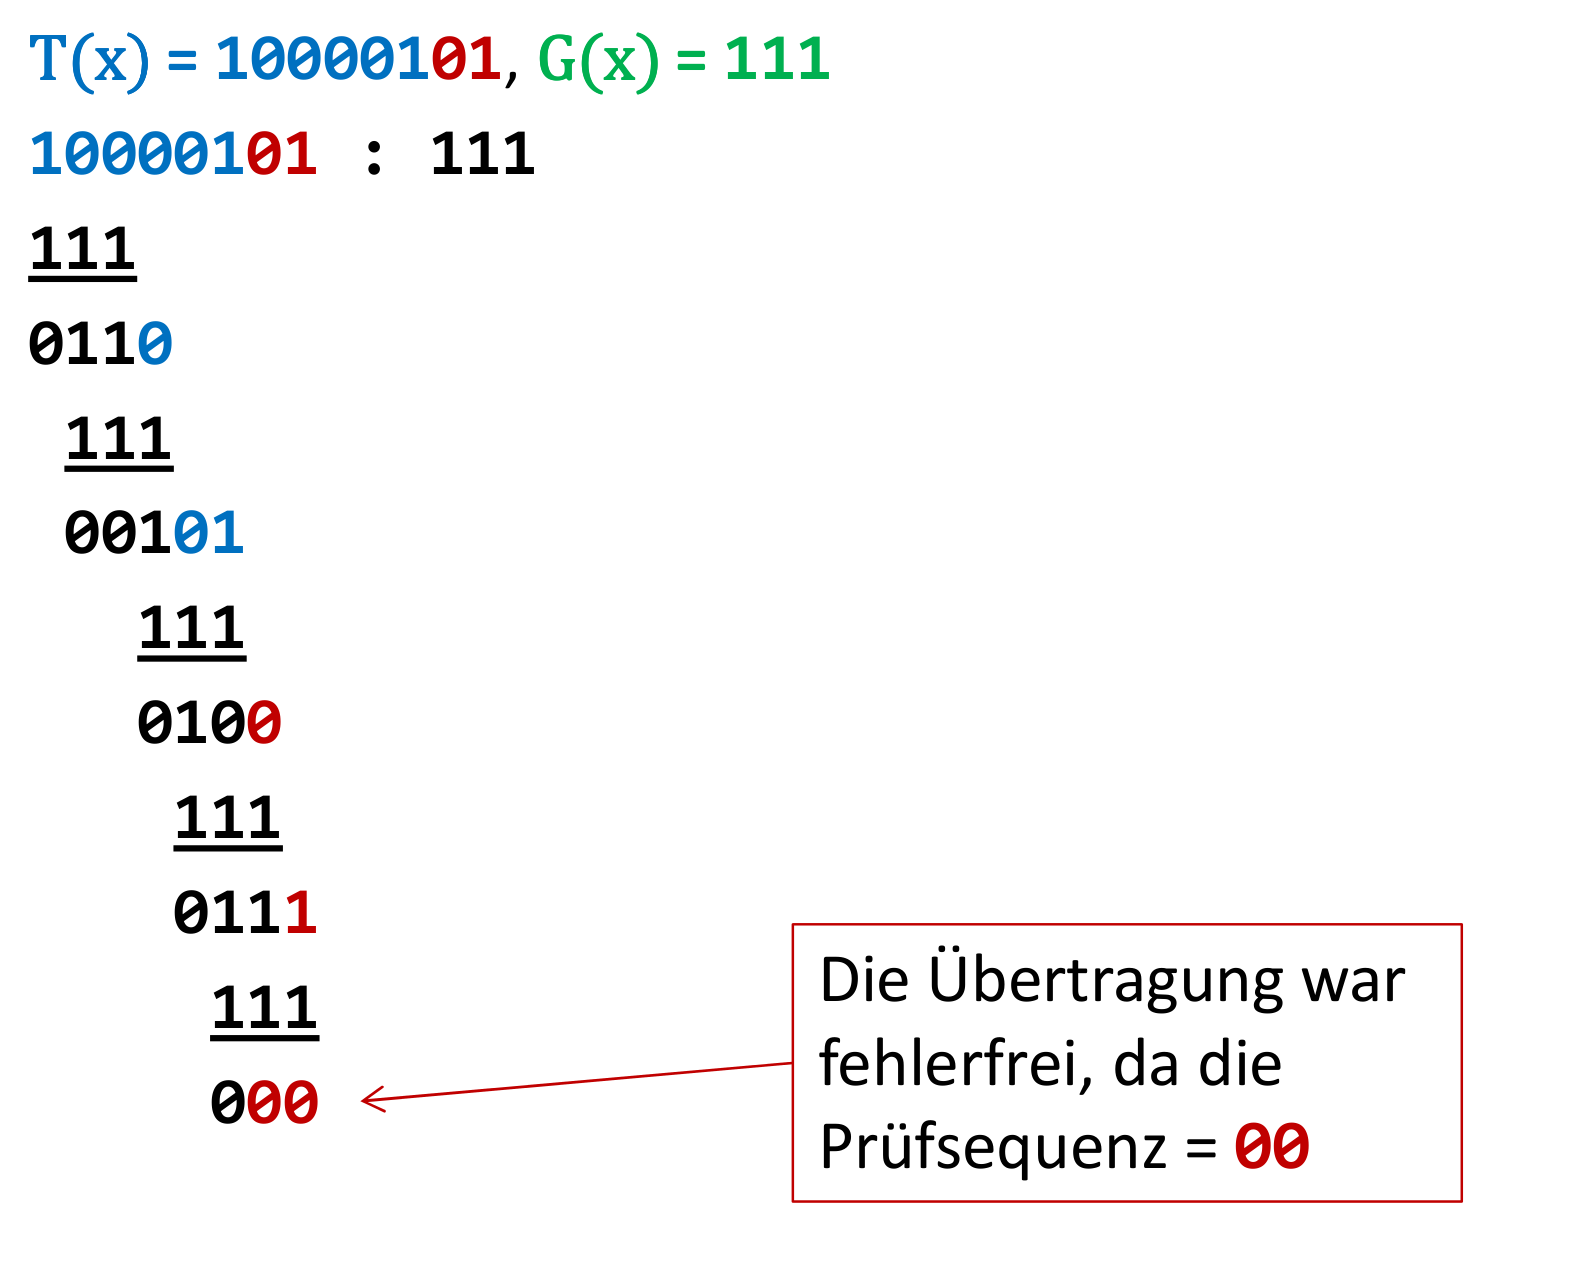
\includegraphics[width=8cm]{images/CRC/crc-enc.png}  \\
\end{tabular}

\subsection{CRC in der Praxis}
\begin{tabular}{|c|c|c|}
\hline \textbf{Bezeichnung} & \textbf{Polynom} & \textbf{Verwendung} \\
\hline CRC-8-CCITT & 0x107 &  ATM, ISDN\\
\hline CRC-16-CCIT & 0x11021 & Bluetooth, SD-Card \\
\hline  CRC-16 & 0x18005  &  Modbus, USB\\
\hline  CRC-32 & 0x104C11DB7 & Ethernet, ZIP, Serial ATA, HDLC, PNG, usw. \\
\hline
\end{tabular}

\begin{itemize}
	\item Da das MSB des Polynoms immer 1 ist, wird dieses häufig bei der Beschreibung weggelassen, z.B. 0x8005 statt 0x18005 beim CRC-16
	\item Teilweise wird auch das LSB weggelassen, da dieses ebenfalls immer 1 ist
\end{itemize}

\textbf{Softwareimplementationen}
\begin{itemize}
	\item Bit um Bit werden berechnet gemäss vorherigem Beispiel
	\item Werte werden vorberechnet und in einer Tabelle abgelegt
\end{itemize}

\textbf{Hardwareimplementationen}
\begin{itemize}
	\item Linear rückgekoppeltes Schieberegister (Linear feedback shift register, LFSR) (siehe \ref{sec:LFSR})
\end{itemize}

\textbf{Breite des Polynoms}
\begin{multicols}{2}
\begin{itemize}
	\item Die CRC-Polynome haben üblicherweise eine Breite von $(x \cdot 8 + 1)$, z.B. 9
	\item Das oberste Bit des Polynoms ist immer eine 1
\end{itemize}
\vfill\null
\columnbreak
\begin{center}
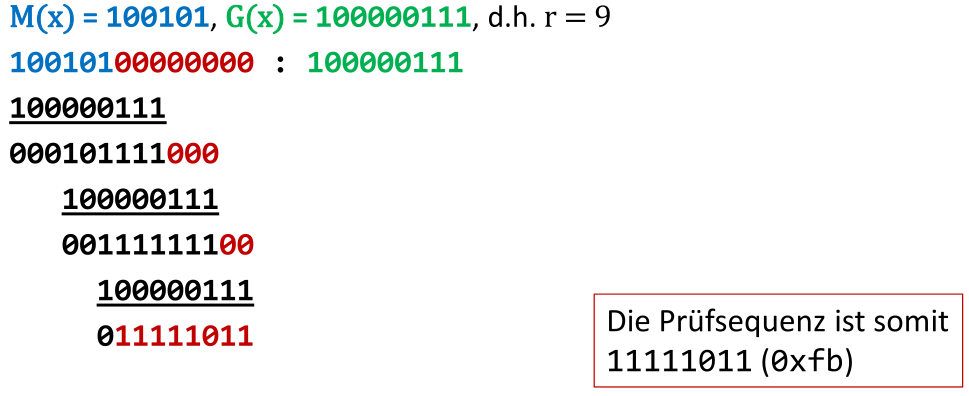
\includegraphics[width=0.8\linewidth]{images/CRC/polynomBreite}
\end{center}
\end{multicols}

\textbf{Die XOR-Operation}
\begin{multicols}{2}
\begin{itemize}
	\item Eine XOR-Operation mit dem Remainder wird nur dann durchgeführt, wenn das oberste Bit des Remainders eine 1 ist, d.h. das oberste Bit des Resultats ist	immer 0.
\end{itemize}
\vfill\null
\columnbreak
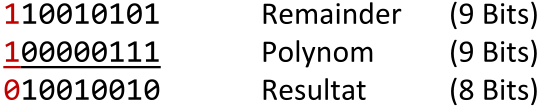
\includegraphics[width=0.8\linewidth]{images/CRC/xor}
\end{multicols}
\begin{itemize}
\item Wenn das Resultat schon im Voraus bekannt ist, muss es auch nicht berechnet werden
\begin{itemize}
	\item Das oberste Bit des Polynoms wird nicht gespeichert, d.h. statt dem eigentlichen Polynom 0x107 (9 Bits) wird nur 0x07 (8 Bits) verwendet
	\item Wenn beim Remainder das oberste Bit eine 1 ist, dann wird der Remainder zuerst um 1 nach links geschoben, und anschliessend mit dem (hier) 8 Bit breiten Polynom eine XOR-Verknüpfung durchgeführt
\end{itemize}
\end{itemize}

\subsection{Implementation}
\subsubsection{Bit by Bit}
 \lstinputlisting[language=C]{code/bitbybit.c}

\textbf{Nachteile}
\begin{itemize}
	\item Jedes Bit wird einzeln behandelt
	\begin{itemize}
		\item Pro Bit: AND, CMP, BNE, SHL, XOR
		\item Sehr aufwendig
	\end{itemize}
	\item Langsam
\end{itemize}


\subsubsection{Tabelle}
\textbf{Ansatz}
\begin{itemize}
	\item Ein Byte hat 256 mögliche Werte, für jeden dieser Werte ist der dazugehörige CRC definiert. Dieser Wert liegt in einer Tabelle vor.
	\item Dadurch erzielt man eine Geschwindigkeitssteigerung um den Faktor 8
	\item Die Kosten dafür sind der Speicherbedarf für die Tabelle (bei einem 8 Bit breiten CRC-Polynom 256 Bytes)
\end{itemize}
\lstinputlisting[language=C]{code/crcfast.c}

\subsection{Linear-Feedback Shift Register (LFSR)}
\label{sec:LFSR}
\begin{itemize}
	\item Ein linear rückgekoppeltes Schieberegister (LFSR) ist ein Schieberegister, dessen Eingang eine lineare Funktion seines vorherigen Zustandes ist.
	\item Ein LFSR besteht aus D-Flip-Flops (Schieberegister), meist mit Rückführungen über XORs.
	\item Mit einem linear rückgekoppelten Schieberegister kann ein CRC in Hardware implementiert werden.
	\item Mit einem LFSR kann auch ein deterministischer Pseudo Random Number Generator erzeugt werden.
	\item Da ein LFSR eine Hardwareschaltung ist, muss nicht auf eine Byte-Orientierung geachtet werden.
	\item Den Initialzustand des Schieberegisters nennt man Seed.
	\item Die Bitpositionen, welche den nächsten Zustand beeinflussen, nennt man Taps.
\end{itemize}

\subsubsection{Fibonacci LFSR}
\begin{itemize}
	\item Das Fibonacci LFSR ist eine (naheliegende) Struktur eines LFSRs.
	\item Die Taps in diesem Beispiel sind [16,14,13,11].
	\item Das Generatorpolynom G(x) lautet dann $1 + x^{11} + x^{13} + x^{14} + x^{16}$
	\item G(x) = 1011010000000001 = 0xB401
	\item Ganz links ist der Input, ganz rechts der Output
	\item Wenn dieses LFSR als CRC verwendet wird, braucht es ganz links nochmals ein XOR, an dem der Bitstream hineingeführt wird.
\end{itemize}
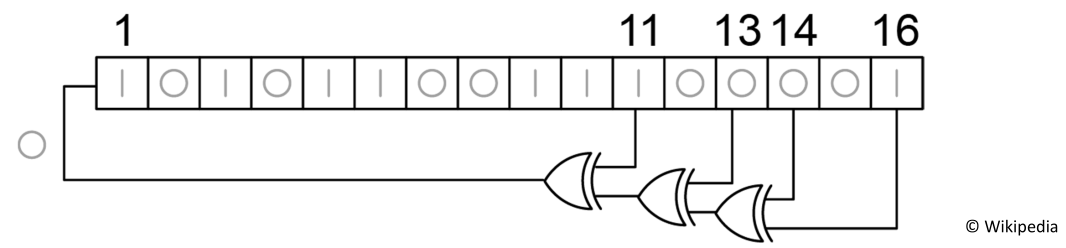
\includegraphics[width=0.6\linewidth]{images/CRC/lfsr}

\subsubsection{Hardware Accelerators in $\mu$C auf Basis eines LFSR}
\begin{itemize}
	\item TI MSP432:
	\begin{itemize}
		\item liefert nur zwei fixe CRCs
		\begin{itemize}
			\item CRC16: CRC-CCITT
			\item CRC32: CRC32-ISO3309
		\end{itemize}
	\end{itemize}
	\item ST STM32
	\begin{itemize}
		\item liefert konfigurierbare CRCs
		\item Die maximale Breite des Schieberegisters ist 32 Bit
		\item Das Polynom (Breite, Taps) kann frei programmiert werden über ein Register, d.h. jedes beliebige Polynom bis maximal 32 Bits ist konfigurierbar.
	\end{itemize}
\end{itemize}
